\documentclass[sigconf]{acmart}

\def\BibTeX{{\rm B\kern-.05em{\sc i\kern-.025em b}\kern-.08emT\kern-.1667em\lower.7ex\hbox{E}\kern-.125emX}}

% Rights management information. 
% This information is sent to you when you complete the rights form.
% These commands have SAMPLE values in them; it is your responsibility as an author to replace
% the commands and values with those provided to you when you complete the rights form.
%
% These commands are for a PROCEEDINGS abstract or paper.
\copyrightyear{2019}
\acmYear{2019}
\setcopyright{acmlicensed}
\acmConference[KDD '19]{KDD '19: 25th ACM SIGKDD Conference on Knowledge Discovery and Data Mining}{August 04--08, 2019}{Anchorage, AK}
\acmBooktitle{KDD '19: 25th ACM SIGKDD Conference on Knowledge Discovery and Data Mining, August 04--08, 2019, Anchorage, AK}
\acmPrice{15.00}
\acmDOI{10.1145/1122445.1122456}
\acmISBN{978-1-4503-9999-9/18/06}

%
% Submission ID. 
% Use this when submitting an article to a sponsored event. You'll receive a unique submission ID from the organizers
% of the event, and this ID should be used as the parameter to this command.
%\acmSubmissionID{123-A56-BU3}

\usepackage{color}
\usepackage{enumitem}
\usepackage{fancyvrb}
\usepackage{multirow}
\usepackage{tabularx}
\usepackage{tabulary}

\definecolor{light-gray}{gray}{0.95}

\newcommand{\naive}{Na\"ive }

\begin{document}

\title{Automated Analysis of Public Health Laboratory Test Results}

\author{William Lu}
\email{williamlu2015@outlook.com}
\affiliation{
    \institution{University of British Columbia}
    \city{Vancouver}
    \state{British Columbia}
    \country{Canada}
}

\author{Sizhe Chen}
\email{joychen0510@gmail.com}
\affiliation{
    \institution{University of British Columbia}
    \city{Vancouver}
    \state{British Columbia}
    \country{Canada}
}

\author{Kenny Chiu}
\email{chiu.kenny@hotmail.com}
\affiliation{
    \institution{University of British Columbia}
    \city{Vancouver}
    \state{British Columbia}
    \country{Canada}
}

\author{Nilgoon Zarei}
\email{nilgoon.zarei@gmail.com}
\affiliation{
    \institution{University of British Columbia}
    \city{Vancouver}
    \state{British Columbia}
    \country{Canada}
}

\author{Raymond Ng}
\email{rng@cs.ubc.ca}
\affiliation{
    \institution{University of British Columbia}
    \city{Vancouver}
    \state{British Columbia}
    \country{Canada}
}

\renewcommand{\shortauthors}{Lu, Chen, Chiu, Zarei, and Ng}

\begin{abstract}
This study investigates the use of machine learning methods for classifying and extracting structured information from laboratory reports stored as semi-structured point-form English text. This is a novel data format that has not been evaluated in conjunction with machine learning classifiers in previous literature. Our classifiers achieve human-level predictive accuracy on the binary \textit{Test Performed} and 4-class \textit{Test Outcome} labels. We consider symbolic approaches for predicting the highly multi-class \textit{Organism Genus} and \textit{Organism Species} labels. Results are discussed from the viewpoint of interpretability and generalizability to new incoming laboratory reports.
\end{abstract}

\begin{CCSXML}
<ccs2012>
<concept>
<concept_id>10010405.10010444.10010449</concept_id>
<concept_desc>Applied computing~Health informatics</concept_desc>
<concept_significance>500</concept_significance>
</concept>
</ccs2012>
\end{CCSXML}

\ccsdesc[500]{Applied computing~Health informatics}

\keywords{machine learning, data science, natural language processing, text mining, semi-structured text}

\maketitle

\section{Introduction}

An important service provided by public health organizations worldwide is the analysis of population-level disease trends \cite{bc_centre_for_disease_control} \cite{surveillance_strategy_report}. These analyses aid efforts for proactive prevention of communicable diseases and provide insight into the historical patterns of pathogen spread. Population-level disease surveillance is also utilized by public health authorities to identify outbreaks and measure the effectiveness of disease control strategies \cite{surveillance_strategy_report}.

Disease surveillance efforts are heavily data-driven, requiring the extraction of structured information from unstructured or semi-structured data. The volume of data is often extremely large. For example, a previous effort by the British Columbia Centre for Disease Control (BCCDC) to monitor patients infected with Hepatitis C required the manual preparation of an anonymized database containing the health records of 1.5 million patients \cite{janjua2016assessing}. The United States Centers for Disease Control and Prevention (USCDC) receives approximately 20 million laboratory reports annually \cite{surveillance_strategy_report}. The BCCDC's data warehouse contains test results spanning over 20 years, with over 2 million test results produced yearly by the BCCDC's Public Health Microbiology and Reference Laboratory \cite{laboratory_program_highlights}.

Increasingly, semi-structured text is the dominant format of clinical data and lab result descriptions, with typical health documents consisting of approximately 60\% structured information and 40\% free-form text \cite{suominen2014guest} \cite{dalianis2009stockholm}. The task of extracting structured information from semi-structured lab result descriptions is currently being performed manually by domain experts. Due to the large volume of data, this manual processing is expensive to carry out, slow, and error-prone.

In this paper, we present a machine learning approach that has demonstrated success in automating this process, achieving human-level ($>95\%$) accuracy. We work with a subset of the lab result descriptions from the BCCDC's data warehouse, comprised of semi-structured text data. Our approach extracts four structured labels:

\begin{enumerate}
    \item A binary \textit{Test Performed} label describing whether the test was performed
    \item A 4-class \textit{Test Outcome} label describing whether the test result is positive, negative, indeterminate, or missing
    \item A multi-class \textit{Organism Genus} label identifying the organism that tested positive, if any
    \item A multi-class \textit{Organism Species} label identifying the organism that tested positive, if any
\end{enumerate}

To the best of our knowledge, no existing literature evaluates the performance of machine learning classifiers on a dataset similar to ours, where text is semi-structured, consists of English words and abbreviations, contains laboratory terminology and organism names as opposed to purely clinical notes, is written in point-form instead of full sentences, and contains contradictory phrases due to new test results invalidating previous observations. We describe the key aspects of our dataset in greater detail in Section \ref{dataset}.

We begin our paper with a review of previous literature relating to similar data mining tasks. We follow with a specific description of the dataset we used to benchmark the performance of our machine learning classifiers. We then present our machine learning models alongside an evaluation of the results achieved on our validation dataset. We conclude by summarizing the limitations of our research, including remarks about the generalizability of our models to test data.

\section{Related Work}

In 2018, Segura-Bedmar et al. evaluated the performance of standard machine learning classifiers in classifying electronic medical records as either positive (describing a case of anaphylaxis) or negative (not describing such a case) \cite{segura2018predicting}. The classifiers they tested included Multinomial \naive Bayes, Logistic Regression, Random Forest, and Linear Support Vector Machine. All the records used to evaluate the classifiers are written in Spanish, unlike our dataset which consists of English text.

In 2014, Velupillai et al. presented a symbolic assertion-based classifier for detecting whether a disorder described in a snippet of semi-structured clinical text is affirmed, negated, or uncertain \cite{velupillai2014cue}. This is similar to our problem of classifying the \textit{Test Outcome} of a lab result as positive, negative, indeterminate, or missing. However, the problem Velupillai et al. solved differs due to the lack of a ``missing'' class. The researchers specifically aimed to construct a system capable of accurately determining the scope and interpretation of negation words such as ``not'' that appear in the clinical text. Their final natural language processing pipeline achieved an overall F-score of 83\% on a corpus of clinical text written in Swedish.

Jang et al. used hidden Markov models to text mine doctors' notes in 2006 \cite{jang2006text}. The document corpus they worked with contained notes written in a mixture of English and Korean. Their models achieved around 60\%-70\% accuracy and aimed to be robust to unknown phrases not seen in the training corpus. One notable tool they used is \textit{MetaMap}, which annotates input text with medical tags and semantics. MetaMap is also commonly used in other health domains, such as text mining for cancer-related information \cite{spasic2014text}.

In 2014, Kang and Kayaalp explored the problem of extracting laboratory test information from biomedical text \cite{kang2013extracting}. They compared the performance of an original symbolic information extraction system to various machine learning-based NLP systems. Their results showed that well-tailored symbolic approaches may outperform machine learning-based approaches. Kang and Kayaalp used a collection of decision summaries from the U.S. Food and Drug Administration as their document corpus. These summaries are written in natural language, unlike our test result descriptions which are written in point-form. We expect this difference will be significant enough that a symbolic approach to our problem will require more complex logic before it can achieve similar results to theirs.

Hasan et al. evaluated the performance of standard machine learning classifiers for multi-class annotation of text data \cite{hasan2016study}. The dataset they used was a collection of around 11,000 transcripts of clinical interviews between psychologists and adolescents or caregivers. They found that a Support Vector Machine classifier was able to annotate conversational snippets with codes from a 17-class codebook with 70.3\% accuracy, although the accuracy decreased to 53.7\% when a 41-class codebook was used.

In a 2016 study \cite{napolitano2016machine}, Napolitano, Marshall, Hamilton, and Gavin used the k-nearest neighbours machine learning algorithm to text mine surgical pathology reports. Their approach was able to identify chunks of text in the reports that provide information about the morphology of the cancer tumours detected and the final diagnoses.

Two previous studies have compared the performance of machine learning classifiers against an expert-constructed Bayesian classifier for detecting reports of influenza in emergency department free-text reports. One study, performed by Pineda et al. in 2015 \cite{pineda2015comparison}, used a corpus consisting of approximately 31 thousand reports. Class imbalance in the dataset was inconsequential given sufficiently many training examples. Notably, the researchers used a tool named \textit{Topaz}, with similar capabilities as MetaMap, to annotate the corpus with UMLS concepts before training the classifiers. The other study, performed by Ye et al. in 2014 \cite{ye2014influenza}, used a training corpus of approximately 29 thousand reports and a testing corpus of approximately 200 reports. Hand-engineered features produced by a domain expert were found to be superior over automatic annotations from Topaz. In both studies, the researchers found that standard machine learning classifiers, such as logistic regression and machine-parameterized \naive Bayes, dominated over the expert-constructed \naive Bayes-like classifier.

In a 2008 study, Pakhomov, Hanson, Bjornsen, and Smith \cite{pakhomov2008automatic} trained support vector machine classifiers on a corpus of 492 unstructured foot examination reports to classify each report as normal (no medical condition was detected), abnormal (a medical condition was detected), or not assessed. This is similar to our problem of classifying a test's outcome as positive, negative, or missing, although Pakhomov et al.'s dataset lacks an ``indeterminate'' class and consists of completely unstructured text from clinical notes. By combining hand-engineered features constructed by domain experts with features automatically extracted using a bag-of-words tokenization process, the SVM classifiers achieved around 80\% accuracy.

A 2017 study performed by Kang et al. \cite{kang2017detecting} demonstrated the efficacy of machine learning algorithms in identifying negation scopes in a corpus of 800 hospital admission notes and discharge summaries written in Chinese. The researchers' learning algorithm vastly outperformed their baseline hand-crafted negation detector, with the former achieving an F-score of 99\% using word embeddings.

\section{Problem Description and Challenges} \label{dataset}

Our dataset is a subset of the data available in BCCDC's data warehouse, and consists of approximately 950,000 test results. This project is one of four research projects conducted in the 2018 University of British Columbia (UBC) Data Science for Social Good program. The project team consisted of four undergraduate and graduate students working full-time from May 2018 to August 2018, with close supervision from the BCCDC investigators and faculty members from the UBC Data Science Institute. To ensure that the project can be completed within four months, only 950,000 test results were included in the project.

Each test result consists of the original laboratory report, stored as semi-structured text, along with structured metadata stored in additional database columns. The original text of the lab report is referred to as the \textit{result full description} (RFD). An RFD is comprised of multiple \textit{observations} delimited by pipe (``\textbar'') characters, where an observation is a chunk of text that was appended to the RFD at one time. An observation is comprised of multiple pipe-delimited \textit{result descriptions}, each of which is either a code-generated phrase or a free-form text string. Due to the laboratory technician having the option of manually appending free-form text to code-generated phrases, there is no consistent structure that would allow for simple rule-based processing. All the text is written in English, but many results are written in short phrases as opposed to full sentences, and do not conform to standard English syntactical and grammatical rules. All pipe characters are automatically added when the separate \textit{result descriptions} are appended together into the RFD to be stored in the data warehouse.

The metadata accompanying an RFD codifies:

\begin{itemize}
    \item The test key and result key, which uniquely identify the test result in the database table
    \item The test code and test name, which identify the specific test routine that was performed
    \item The test type, including but not limited to culture, antibody, and NAT/PCR types
    \item The ID of the lab system the test result came from
    \item The breakdown of the RFD into its constituent observations and result descriptions
\end{itemize}

Some lab reports in the dataset are results of proficiency tests, which are routine tests performed on known samples to confirm that the lab equipment and processing techniques are producing accurate results. Other lab reports have empty RFD strings, or RFDs consisting purely of a floating-point number such as ``0.016''. All proficiency tests and results with empty or purely numeric RFDs were filtered from the dataset before further analysis was performed, which reduced the size of the dataset to 362,806 test results.

Table \ref{tab:dataset_counts} lists the 20 most frequently occurring unigrams among the RFDs in our dataset. This analysis is case-insensitive, so lowercase and uppercase versions of the same unigram are counted together. Stopwords included in the Python \textit{wordcloud} package's default stop word list are not included in the table. The most frequent unigrams are laboratory terms such as ``specimen'', ``reactive'', and ``infection''. Organism names and abbreviations such as ``hepatitis'' and ``hiv'', and abbreviations such as ``ml'', also appear regularly in the RFDs.

\begin{table}
    \caption{The 20 most frequently occurring unigrams in the corpus of RFDs, along with their occurrence counts.}
    \label{tab:dataset_counts}
    
    \begin{tabular}{ccccc}
        \toprule
        Unigram & Count & \quad & Unigram & Count \\
        \midrule
        specimen & 120,782 & \quad & result & 40,481 \\
        previous & 69,247 & \quad & performed & 40,372 \\
        collected & 66,048 & \quad & immune & 40,254 \\
        reactive & 65,663 & \quad & may & 37,749 \\
        test & 64,213 & \quad & please & 32,125 \\
        infection & 51,743 & \quad & identified & 32,111 \\
        tests & 50,817 & \quad & hiv & 31,787 \\
        hepatitis & 49,629 & \quad & non & 31,020 \\
        completed & 49,165 & \quad & laboratory & 30,937 \\
        detected & 42,269 & \quad & ml & 30,265 \\
        \bottomrule
    \end{tabular}
\end{table}

Examples of the semi-structured RFDs are listed below. All dates have been changed to May 29th, 2017, although their original formats have been preserved:

\begin{enumerate}
    \item \textit{Specimen rejected \textbar\ Test not performed. \textbar\ No evidence of HCV infection.}
    \item \textit{No Bordetella pertussis DNA detected by PCR.}
    \item \textit{Result inconclusive. \textbar\ Culture results to follow. \textbar\ Varicella Zoster Virus \textbar\ `Isolated.'}
    \item \textit{`Organism identified as:' \textbar\ Haemophilus influenzae \textbar\ Biotype \textbar\ \textbar\ non serotypable (non encapsulated)}
\end{enumerate}

Some test results contain spelling, grammatical, and typographical errors, and are thus more challenging for hand-coded rules to process. For example, ``serotype'' is misspelled as ``seretype'' and ``group'' is misspelled as ``froup'' in the RFD below:

\begin{enumerate}[resume]
    \item \textit{BCCDC seretype: non froup 5 \textbar\ Final \textbar\ 29/May/2017 \textbar\ Sputum \textbar\ Streptococcus pneumoniae \textbar\ STUDY}
\end{enumerate}

Another challenge lies in the ambiguous use of the word ``not'', as it could be interpreted as negating the entire test result, negating the current observation, or as part of a subtype of an organism, among many other interpretations:

\begin{enumerate}[resume]
    \item \textit{NEGATIVE for Shiga toxin stx1 and stx2 genes by PCR. \textbar\ Isolate serotyped as: \textbar\ Escherichia coli \textbar\ not \textbar\ O157:H7}
    \item \textit{Isolate not \textbar\ Salmonella species}
\end{enumerate}

A further challenge is the presence of many negative organism names in some test results. For example, the following RFD contains all organisms that multiplex NAT is capable of detecting. However, only Rhinovirus, Enterovirus, and Adenovirus were positive in the actual test:

\begin{enumerate}[resume]
    \item \textit{Rhinovirus or Enterovirus detected by multiplex NAT. \textbar\ \textbar\ Adenovirus detected by multiplex NAT. \textbar\ \textbar\ Multiplex NAT is capable of detecting Influenza A and B, Respiratory Syncytial Virus, Parainfluenza 1, 2, 3, and 4, Rhinovirus, Enterovirus, Adenovirus, Coronaviruses HKU1, NL63, OC43, and 229E, hMetapneumovirus, Bocavirus, C. pneumoniae, L. pneumophila, and M. pneumoniae. \textbar\ \textbar\ MULTIPLE INFECTION DETECTED}
\end{enumerate}

Due to clinical procedures, early conclusions recorded in the lab reports that were invalidated by later tests cannot be erased. Thus, some lab reports contain contradictory information. For example, only Moraxella osloensis is positive in the RFD below, despite the text mentioning Neisseria meningitidis as well:

\begin{enumerate}[resume]
    \item \textit{Organism identified as: \textbar\ Neisseria meningitidis nongroupable \textbar\ Upon further investigation \textbar\ Organism identified as: \textbar\ Moraxella osloensis \textbar\ by 16S rRNA gene sequence analysis.}
\end{enumerate}

Adding to the problem complexity, the most up-to-date information is not always written at the end of the RFD. For example, the test corresponding to the RFD below was not performed, despite the last observation stating the contrary:

\begin{enumerate}[resume]
    \item \textit{TEST NOT PERFORMED \textbar\ Galactomannan testing is valid only for Haematology and lung transplant patients with no recent antifungal exposure \textbar\ Test performed at Provincial Laboratory of Public Health, Edmonton}
\end{enumerate}

Some RFDs contain dates written in various formats, including but not limited to the following:

\begin{enumerate}[resume]
    \item \textit{Hepatitis C tests completed on previous specimen. \textbar\ Collected on 29 May 2017.}
    \item \textit{2+ \textbar\ Acid Fast Bacilli found \textbar\ CORRECTED ON 29/May AT 1132: PREVIOUSLY REPORTED AS No acid fast bacilli found.}
    \item \textit{17/05/29}
\end{enumerate}

In this work, we extract four structured labels from the semi-structured RFDs. The labels and their constituent classes are numbered and summarized in Table \ref{tab:labels_and_classes}. The \textit{Test Performed} label codifies whether a test was successfully performed, with the \textit{Yes} class identifying tests which were performed successfully to completion, and the \textit{No} class identifying tests which were deemed inapplicable, cancelled due to contamination of the specimen sample, or which failed to produce valid results due to a technical issue. The \textit{Test Outcome} label represents whether the organism of interest was detected in the specimen sample, with \textit{Positive} meaning detected, \textit{Negative} meaning not detected, \textit{Indeterminate} meaning no conclusion was reached, and \textit{Missing} meaning the result is unknown due to lack of data. The \textit{Organism Genus} and \textit{Organism Species} labels contain the scientific name of the organism detected in the test.

\begin{table}
    \caption{The labels and classes we extract from the semi-structured data.}
    \label{tab:labels_and_classes}
    
    \begin{tabular}{ccc}
        \toprule
        \# & Label & Classes \\
        \toprule
        \multirow{2}{*}{1} & \multirow{2}{*}{Test Performed} & Yes \\
                           &                                 & No \\
        \midrule
        \multirow{4}{*}{2} & \multirow{4}{*}{Test Outcome} & Positive \\
                           &                               & Negative \\
                           &                               & Indeterminate \\
                           &                               & Missing \\
        \midrule
        3 & Organism Genus & $\approx 30$ classes (and counting) \\
        \midrule
        4 & Organism Species & $\approx 160$ classes (and counting) \\
        \bottomrule
    \end{tabular}
\end{table}

The dataset has been partially labeled by a domain expert. Each label has a different number of labeled rows, summarized in Table \ref{tab:dataset_labeled}.

\begin{table}
    \caption{The amount of labeled data for each label, expressed in number of rows and percentage of the full dataset.}
    \label{tab:dataset_labeled}
    
    \setlength\tymin{2.5cm}
    \begin{tabulary}{\linewidth}{CCC}
        \toprule
        Label & Number of labeled rows & Percentage of labeled rows \\
        \midrule
        Test Performed & 362,806 & 100\% \\
        Test Outcome & 115,347 & 31.79\% \\
        Organism Genus & 40,289 & 11.10\% \\
        Organism Species & 40,289 & 11.10\% \\
        \bottomrule
    \end{tabulary}
\end{table}

Table \ref{tab:tp_labeled} summarizes the class breakdown for the labeled \textit{Test Performed} rows. Notably, the labeled data exhibits severe class imbalance, with the \textit{Yes} class dominating in row count by an order of magnitude. We also note the presence of a \textit{Pending} class, which is outside the scope of our study. We filter all \textit{Pending} rows from our labeled data before doing further analysis.

Moderate class imbalance is present in the labeled \textit{Test Outcome} rows, as summarized in Table \ref{tab:to_labeled}. The \textit{Organism Genus} label exhibits severe class imbalance. The two largest classes, \textit{Not Found} and \textit{Hepatitis C Virus}, respectively represent 46\% and 21\% of the labeled dataset. Each of the two smallest classes, \textit{Treponema} and \textit{Trichomas}, contains around 40 labeled examples and accounts for approximately 0.1\% of the labeled data. The \textit{Organism Species} label suffers from an extreme lack of labeled data for its smallest classes, each of which has only 1 labeled example. Both organism-related labels are constantly gaining new classes due to previously unseen organisms being reported in new test results.

\begin{table}
    \caption{Class breakdown for the labeled \textit{Test Performed} data. Percentages are with respect to all labeled \textit{Test Performed} rows.}
    \label{tab:tp_labeled}

    \begin{tabular}{ccc}
        \toprule
        Class & Number of rows & Percentage of rows \\
        \midrule
        Yes & 340,474 & 93.84\% \\
        No & 22,114 & 6.10\% \\
        Pending & 218 & 0.06\% \\
        \bottomrule
    \end{tabular}
\end{table}

\begin{table}
    \caption{Class breakdown for the labeled \textit{Test Outcome} data. Percentages are with respect to all labeled \textit{Test Outcome} rows.}
    \label{tab:to_labeled}
    
    \begin{tabular}{ccc}
        \toprule
        Class & Number of rows & Percentage of rows \\
        \midrule
        Positive & 19,249 & 16.69\% \\
        Negative & 15,268 & 13.24\% \\
        Indeterminate & 1,453 & 1.26\% \\
        Missing & 79,377 & 68.82\% \\
        \bottomrule
    \end{tabular}
\end{table}

\section{Approach}

\subsection{Preprocessing}

We clean our dataset to remove unnecessary tokens and resolve inconsistencies that would hinder the performance of our classifiers. We convert all existing labels in our dataset to lowercase for consistency, since they appear in both title-case (e.g. ``Positive'') and lower-case (e.g. ``positive'') versions. Using a regular expression, we remove all characters that are not alphanumeric characters, spaces, or pipes from the RFDs. We replace all standalone numbers, such as ``16'' or ``15.09'', in the RFDs with the ``\_NUMBER\_'' token to prevent our classifiers from fitting to specific numbers. We do not replace dates with a ``\_DATE\_'' token due to the difficulty of identifying all possible date formats that appear in the RFDs.

\subsection{Machine learning approach}

We use a machine learning approach for classifying the \textit{Test Performed}, \textit{Test Outcome}, and \textit{Organism Genus} labels. We extract features from the RFDs using scikit-learn's bag-of-words count vectorizer. For the \textit{Test Performed} label, we extract unigrams, bigrams, and trigrams due to ``Test Not Performed'' being a consistently important feature for predicting this label. We exclude all features that occur in less than 10 RFDs to speed up computation. For the \textit{Test Outcome} label, we extract only unigrams, in order to speed up computation and reduce correlation between features in the feature space. For \textit{Test Outcome}, we only exclude features that occur in less than 5 RFDs. For the \textit{Organism Genus} label, we extract unigrams and we do not exclude any features on the basis of document frequency due to important organism names appearing infrequently. We experimented with TF-IDF feature representations and found that they did not improve classifier performance.

We use scikit-learn implementations of standard machine learning classifiers including \naive Bayes (NB), Logistic Regression (LR), Random Forest with 100 trees (RF), and Support Vector Machine with linear kernel (SVM). Since we are using supervised machine learning algorithms, our results for each label are obtained on the subset of labeled data for that label. We evaluate the performance of our classifiers using 5-fold cross validation. For each classifier, we use the mean accuracy obtained over the 5 folds as a performance metric. We also report the cumulative confusion matrix obtained over the 5 folds, and class-wise precision and recall, for the SVM classifier. For the \textit{Test Performed} and \textit{Test Outcome} labels, we carry out an error analysis and report common RFD patterns that are frequently misclassified by the SVM classifier.

We investigate which features are deemed by our models to be most influential in making predictions. For the \textit{Test Performed} label, we retrain our LR classifier on the full labeled dataset and report the 10 most negative and 10 most positive weighted features along with their regression weights. For the \textit{Test Outcome} and \textit{Organism Genus} labels, we retrain our RF classifier on the full labeled dataset and report the 10 features with the highest importance scores.

We experiment with class reweighing as a potential solution to class imbalance in the \textit{Test Performed} training set. We use the \textit{multi\_class=``balanced''} parameter on scikit-learn's SVM classifier implementation, and we report the differences in the class-wise precision and recall scores compared with the results obtained by the non-balanced SVM classifier.

\subsection{Symbolic approach}

We consider a symbolic approach for classifying the \textit{Organism Genus} and \textit{Organism Species} labels. The large number of classes, the lack of labeled data for the minority classes, and the constant addition of new classes would render machine learning algorithms ineffective. Although symbolic algorithms necessitate more manual hard-coding of domain rules, their classification decisions are completely transparent and their parameters are easier to modify and interpret than those of machine learning algorithms. We make use of MetaMap, an application that annotates free text with tags from a database of UMLS biomedical terms and concepts. MetaMap is capable of mapping abbreviations or common names that appear in the RFDs to the corresponding scientific names. For each RFD in our dataset, we acquire from MetaMap a list of organism concepts that were detected. If the generic concepts ``Bacteria'' and ``Virus'' are present, we remove them from the list. We call this final list the \textit{candidates} list for the RFD.

Our symbolic classifiers have training and prediction phases. During the training phase, the classifier stores a dictionary of existing classes seen in the labeled dataset. The \textit{Organism Genus} classifier stores a set of genus names, excluding the special class ``Not Found''. The \textit{Organism Species} classifier stores a mapping between genus names and possible species names for each genus, again excluding the special class ``Not Found''.

During the \textit{Organism Genus} classifier's prediction phase, the classifier consults an SVM \textit{Test Outcome} classifier. If the predicted test outcome is ``negative'', or if the RFD's candidates list is empty, the \textit{Organism Genus} classifier returns ``Not Found'' in accordance with the domain rules. Otherwise, for each candidate in the list, the classifier considers each prefix of that candidate. If a prefix is present in the classifier's dictionary, the classifier returns the prefix as its final prediction. Prefixes are taken at the word level. For example, the prefixes for the candidate ``hepatitis c virus'' are \{``hepatitis c virus'', ``hepatitis c'', ``hepatitis''\}. If no match is found after examining all candidates, the classifier returns an arbitrary candidate in the list.

The \textit{Organism Species} classifier uses a similar prediction algorithm. It consults an SVM \textit{Organism Genus} classifier and returns ``Not Found'' if the predicted genus is ``Not Found'', if the predicted genus is not in its own dictionary, or if the candidates list is empty. Otherwise, the algorithm considers each word-level prefix of each candidate. If a prefix is in the dictionary's set of allowable species names for the predicted genus name, the algorithm returns the prefix as its final prediction. If no match is found after examining all candidates, the algorithm returns an arbitrary candidate.

\section{Results and Discussion} \label{results_and_discussion}

\subsection{Label 1: \textit{Test Performed}}

Our \textit{Test Performed} classifiers achieve high classification accuracies. \naive Bayes achieves approximately 94\% accuracy while all other classifiers achieve approximately 98\% accuracy, as summarized in Table \ref{tab:tp_accuracies}. From the logistic regression weights listed in Figure \ref{fig:tp_lr_features}, we note that the trigram ``test not performed'' is consistently the strongest indicator of the \textit{Test Performed} label. Further, the features ``sample not received'' and ``no sample received'' are strong indicators that the test was not performed. Curiously, the strongest predictor for the \textit{Yes} class is ``test not done''. We caution that the feature space contains pairs of correlated features, such as ``not performed'' and ``test not performed''. Thus, the regression weights may not be perfectly indicative of feature importance, although they provide a reasonable approximation.

\begin{table}
    \caption{Accuracy scores obtained on the \textit{Test Performed} label.}
    \label{tab:tp_accuracies}
    
    \centering
    \begin{tabular}{ccc}
        \toprule
        Classifier & Accuracy \\
        \midrule
        \naive Bayes & 93.96\% \\
        Logistic Regression & 98.58\% \\
        Random Forest & 98.60\% \\
        Support Vector Machine & 98.54\% \\
        \bottomrule
    \end{tabular}
\end{table}

\begin{figure}
    \centering
    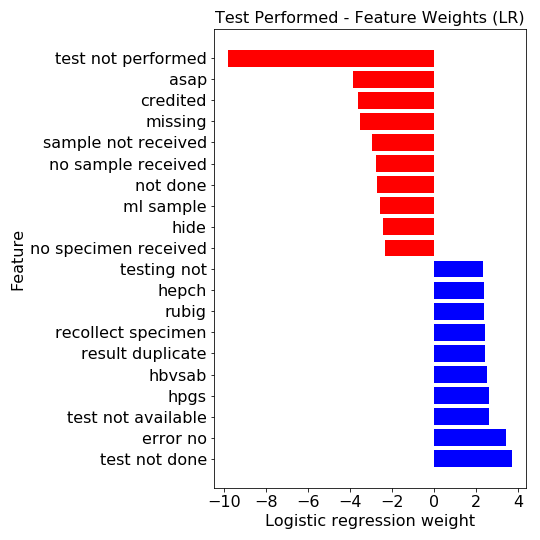
\includegraphics[width=\linewidth]{tp_lr_features.png}
    \caption{The 10 most negative and 10 most positive weighted features in the logistic regression \textit{Test Performed} classifier.}
    \Description{Most negative features: ``test not performed'', ``asap'', ``credited'', ``missing'', ``sample not received'', ``not done'', ``ml sample'', ``hide'', ``no specimen received''. Most positive features: ``test not done'', ``error no'', ``test not available'', ``hpgs'', ``hbvsab'', ``result duplicate'', ``recollect specimen'', ``rubig'', ``hepch'', ``testing not''.}
    \label{fig:tp_lr_features}
\end{figure}

Analysis of the SVM classifier's confusion matrix (Table \ref{tab:tp_svm_confusion}) shows that class imbalance is causing our classifiers to be biased towards the majority class \textit{Yes}. In particular, we achieve a 84.59\% recall score for the \textit{No} class, which is considerably lower than the other precision and recall scores, which are in the nineties. Class reweighing reduced false positives (true label ``No'', predicted as ``Yes'') at the expense of introducing false negatives (true label ``Yes'', predicted as ``No''): although the minority class's recall score increased to 91.08\%, the minority class's precision score decreased significantly to 64.61\%. Consultation with a domain expert revealed that, from a surveillance point of view, false positives are more acceptable than false negatives, particularly when the diseases under surveillance are not considered rare. Thus, we retain our original classifiers in our final production code, opting not to use class reweighing.

\begin{table}
    \caption{The confusion matrix obtained from the SVM \textit{Test Performed} classifier, without class reweighing.}
    \label{tab:tp_svm_confusion}
    
    \begin{tabular}{cccc}
        \toprule
        & Predicted \textit{Yes} & Predicted \textit{No} & Recall \\
        \midrule
        True \textit{Yes} & 338581 & 1893 & 99.44\% \\
        True \textit{No} & 3407 & 18707 & 84.59\% \\
        Precision & 99.00\% & 90.81\% & \\
        \bottomrule
    \end{tabular}
\end{table}

Table \ref{tab:tp_svm_error} lists a sample of rows misclassified by SVM. For confidentiality, the original specimen number in the first row has been replaced with K12345. Error analysis reveals that a significant number of misclassified rows are semantically ambiguous, with the text seemingly contradicting the true label. For example, the RFD ``Insufficient material provided for examination'' has true label \textit{Yes}. Furthermore, some rows, such as ``MYCOF FROM SPH'' and ``Liver'', do not provide enough information to realistically discern the correct \textit{Test Performed} class. Consultation with a domain expert revealed that the true labels in these cases are assigned according to a set of structured flags, which are outside the scope of our study and not used as features in our classifiers. Some other rows contain test metadata information instead of actual test results, and have been labeled ``Yes'' to reflect their successful entry into the data warehouse.

\begin{table}
    \caption{Rows misclassified by the SVM \textit{Test Performed} classifier.}
    \label{tab:tp_svm_error}
    
    \centering
    \setlength\tymin{0.7cm}
    \begin{tabulary}{\linewidth}{CCC}
        \toprule
        Result full description & True label & Pred. label \\
        \toprule
        Insufficient material provided for examination \textbar\ See specimen K12345 for MTD result & Yes & No \\
        \midrule
        MYCOF FROM SPH & Yes & No \\
        \midrule
        Nonreactive \textbar\ INTERPRETATION \textbar\ No evidence of HTLV I or II infection & No & Yes \\
        \midrule
        NOT DONE \textbar\ Unsatisfactory Specimen wrapped in tissue or paper Please submit another specimen instructing patient to expectorate directly into the jar & Yes & No \\
        \midrule
        Liver & No & Yes \\
        \bottomrule
    \end{tabulary}
\end{table}

\subsection{Label 2: \textit{Test Outcome}}

Our machine learning classifiers achieve high ($> 95\%$) accuracies on \textit{Test Outcome}, as summarized in Table \ref{tab:to_accuracies}. According to the SVM confusion matrix (Table \ref{tab:4cto_svm_confusion}) and the corresponding precision and recall scores (Table \ref{tab:4cto_svm_summary}), class imbalance does not appear to be affecting the results of the minority class \textit{Indeterminate} by a large margin, with its precision score being 89.78\% and its recall score being 88.23\%.

\begin{table}
    \caption{Accuracy scores obtained on the \textit{Test Outcome} label.}
    \label{tab:to_accuracies}
    
    \centering
    \begin{tabular}{ccc}
        \toprule
        Classifier & Accuracy \\
        \midrule
        \naive Bayes & 92.33\% \\
        Logistic Regression & 99.14\% \\
        Random Forest & 99.24\% \\
        Support Vector Machine & 99.17\% \\
        \bottomrule
    \end{tabular}
\end{table}

\begin{table}
    \caption{The confusion matrix obtained from the SVM \textit{Test Outcome} classifier.}
    \label{tab:4cto_svm_confusion}
    
    \begin{tabularx}{\linewidth}{cccccc}
        \toprule
        & Pred. \textit{Pos.} & Pred. \textit{Neg.} & Pred. \textit{Ind.} & Pred. \textit{Mis.} \\
        \midrule
        True \textit{Pos.} & 19034 & 74 & 36 & 105 \\
        True \textit{Neg.} & 53 & 15037 & 49 & 129 \\
        True \textit{Ind.} & 35 & 76 & 1282 & 60 \\
        True \textit{Mis.} & 101 & 178 & 61 & 79037 \\
        \bottomrule
    \end{tabularx}
\end{table}

\begin{table}
    \caption{The class-wise precision and recall scores obtained from the SVM \textit{Test Outcome} classifier.}
    \label{tab:4cto_svm_summary}
    
    \begin{tabular}{ccc}
        \toprule
        Class & Precision & Recall \\
        \midrule
        Positive & 99.02\% & 98.88\% \\
        Negative & 97.87\% & 98.49\% \\
        Indeterminate & 89.78\% & 88.23\% \\
        Missing & 99.63\% & 99.57\% \\
        \bottomrule
    \end{tabular}
\end{table}

Figure \ref{fig:4cto_rf_features} lists the most important features for predicting \textit{Test Outcome} according to the RF classifier. Notably, hepatitis-B-related abbreviations, namely ``hbsag'' and ``hbv'', are instrumental in predicting the test outcome, implying that our \textit{Test Outcome} classifiers are fitting to specific organisms due to the presence of a large number of hepatitis-B-related rows in our dataset. This may result in our classifiers mislabeling rows containing different organism names. We discuss potential solutions in Section \ref{limitations_and_future_work}.

\begin{figure}
    \centering
    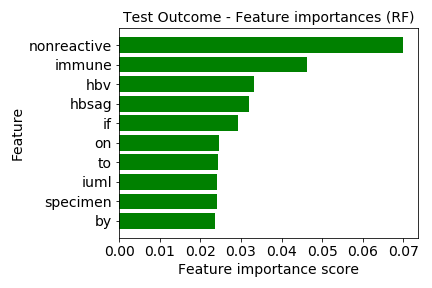
\includegraphics[width=\linewidth]{4cto_rf_features.png}
    \caption{The 10 most important features for test outcome according to RF.}
    \Description{Most important features: nonreactive, immune, hbv, hbsag, if, on, to, iuml, specimen, by.}
    \label{fig:4cto_rf_features}
\end{figure}

Table \ref{tab:bto_svm_error} lists a sample of RFDs misclassified by the \textit{Test Outcome} SVM classifier. The misclassified RFDs almost exclusively contain contradictory information due to the initial result having been invalidated or updated at a later date. This implies that our classifiers are still struggling to understand negation scope. Nevertheless, many RFDs containing contradictions are indeed classified correctly by our current SVM classifier, showing that a linear classifier is able to produce reasonably accurate predictions.

\begin{table}
    \caption{Rows misclassified by the SVM \textit{Test Outcome} classifier.}
    \label{tab:bto_svm_error}
    
    \centering
    \setlength\tymin{1.2cm}
    \begin{tabulary}{\linewidth}{CCC}
        \toprule
        Result full description & True label & Pred. label \\
        \toprule
        Bordetella pertussis DNA detected by PCR \textbar\ CORRECTED ON 29May AT \_NUMBER\_ PREVIOUSLY REPORTED AS No Bordetella pertussis DNA detected by PCR \textbar\ Culture results to follow & Positive & Negative \\
        \midrule
        Neisseria gonorrhoeae \textbar\ POSITIVE \textbar\ Susceptibility results to follow \textbar\ Upon further investigation organism isolated is not Neisseria gonorrheae \textbar\ Please disregard report sent \_NUMBER\_ \textbar\ Corrected Report \textbar\ No Neisseria gonorrhoeae isolated & Negative & Positive \\
        \midrule
        No diplococci resembling Neisseria gonorrhoeae present \textbar\ CORRECTED ON 29May AT \_NUMBER\_ PREVIOUSLY REPORTED AS Diplococci resembling Neisseria gonorrhoeae present \textbar\ Polymorphs polynucleated cells \_NUMBER\_ & Negative & Positive \\
        \midrule
        HIGHLY SUSPICIOUS FOR N GONORRHOEAE BUT DOES NOT MEET ALL OF THE CRITERIA FOR A POSITIVE RESULT & Missing & Positive \\
        \bottomrule
    \end{tabulary}
\end{table}

\subsection{Label 3: \textit{Organism Genus}}

For the \textit{Organism Genus} label, our machine learning classifiers achieve around 98\% accuracy and our symbolic algorithm achieves around 89\% accuracy (Table \ref{tab:og_accuracies}). Analysis of the class-wise precision and recall scores achieved by the SVM and symbolic classifiers (Figures \ref{fig:ogc_precision} and \ref{fig:ogc_recall}) show that the symbolic algorithm performs worse in almost all cases compared to the SVM classifier. The most important features for predicting \textit{Organism Genus}, according to our RF classifier, are summarized in Figure \ref{fig:ogml_rf_alt_features}. Notably, only four of these features (``salmonella'', ``streptococcus'', ``hcv'', and ``coli'') refer to specific organisms. Due to the difficulty of interpreting the rest of the selected features, we prefer the symbolic classifier for its transparency and explicit reliance on UMLS organism concept tags. We note that it is possible to extend the symbolic algorithm with more domain rules to significantly improve its accuracy.

\begin{table}
    \caption{Accuracy scores obtained on the \textit{Organism Genus} label.}
    \label{tab:og_accuracies}
    
    \centering
    \begin{tabular}{ccc}
        \toprule
        Classifier & Accuracy \\
        \midrule
        \naive Bayes & 91.52\% \\
        Logistic regression & 98.06\% \\
        Random forest & 97.31\% \\
        Support vector machine & 98.18\% \\
        Symbolic & 89.84\% \\
        \bottomrule
    \end{tabular}
\end{table}

\begin{figure}
    \centering
    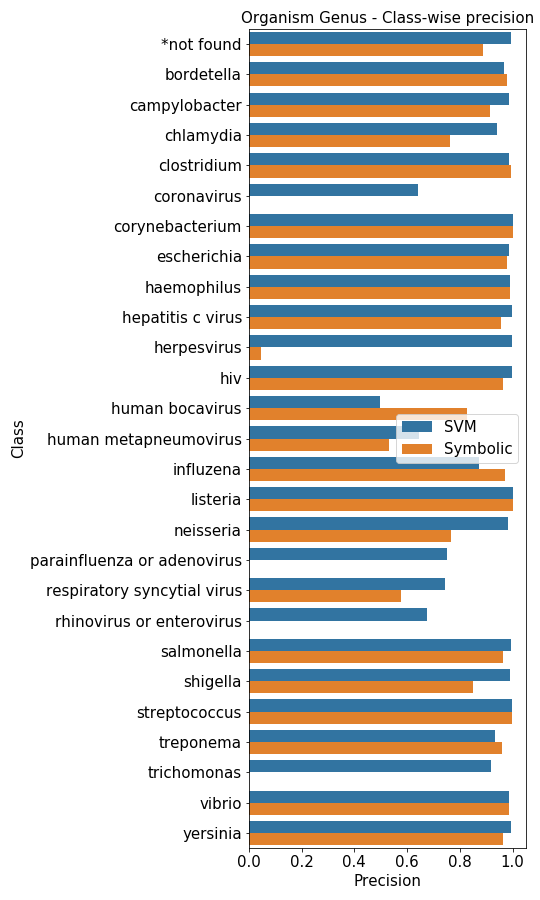
\includegraphics[width=\linewidth]{ogc_precision.png}
    \caption{Class-wise precision scores achieved by the \textit{Organism Genus} SVM and symbolic classifiers.}
    \Description{The SVM classifier outperforms the symbolic classifier in almost all cases.}
    \label{fig:ogc_precision}
\end{figure}

\begin{figure}
    \centering
    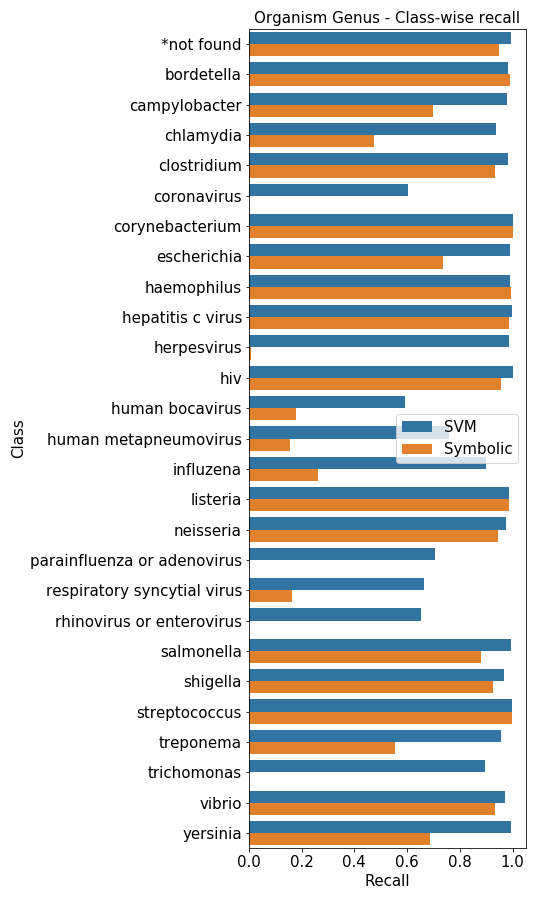
\includegraphics[width=\linewidth]{ogc_recall.png}
    \caption{Class-wise recall scores achieved by the \textit{Organism Genus} SVM and symbolic classifiers.}
    \Description{The SVM classifier outperforms the symbolic classifier in almost all cases.}
    \label{fig:ogc_recall}
\end{figure}

\begin{figure}
    \centering
    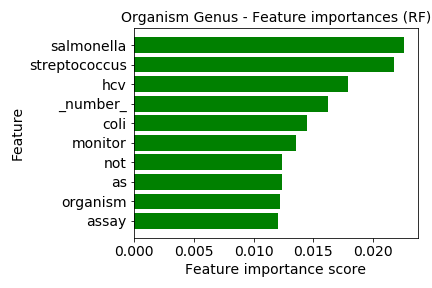
\includegraphics[width=\linewidth]{ogml_rf_alt_features.png}
    \caption{The 10 most important features for predicting organism genus using RF.}
    \Description{Most important features: salmonella, streptococcus, hcv, _number_, coli, monitor, not, as, organism, assay}
    \label{fig:ogml_rf_alt_features}
\end{figure}

\subsection{Label 4: \textit{Organism Species}}

We obtain 61.54\% accuracy on \textit{Organism Species} using our symbolic classifier. Notably, out of the 169 classes, 59 classes have precision 0\% and 78 classes have precision 100\%, and 59 classes have recall 0\% and 61 classes have recall 100\%. Investigation revealed that the classes with 0\% precision and recall are mostly subtypes of Hepatitis C, such as ``hepatitis c virus genotype 1''. Our classifier mislabels all rows in these classes due to the candidate lists from MetaMap not containing genotype information.

We note that MetaMap's annotation process is slow, taking approximately 12 hours to annotate one million RFDs on a Microsoft Windows 2008 R2 virtual server with 8 GB of RAM and 2 Intel Xeon cores clocked at 3.06 GHz speed.

\section{Limitations and Future Work} \label{limitations_and_future_work}

Due to organizational and patient privacy and confidentiality policies, we are only provided with data from the BCCDC to use in our analysis. As such, our results may not generalize completely to datasets from other institutions. In particular, other public health organizations may use different coding schemes, different computer-generated lexica, different data entry practices, or have data with different class distributions. Notwithstanding, we expect that datasets similar to ours, in that they are written in English point-form, contain laboratory terminology and organism names and abbreviations, and are semi-structured due to a combination of computer-generated and free-form text, should achieve comparable performance when classifying labels similar to ours.

We note in Section \ref{results_and_discussion} that the \textit{Test Outcome} machine learning classifiers are making predictions based in part on specific organism abbreviations that appear to be irrelevant to predicting test outcome. Additionally, important structured metadata such as flags encoding \textit{Test Performed} knowledge are lacking from our dataset, and are therefore not used as features in our classifiers. Future goals may focus on including relevant structured metadata as input features to our classifiers. Further work may consider the usage of MetaMap for removing specific organism concepts from the RFDs before feeding them to the \textit{Test Outcome} classifiers.

We note that the \textit{Organism Species} symbolic classifier is failing to correctly classify any rows in approximately 50 classes due to the MetaMap organism candidates not aligning with the class names. A future version of this classifier may include a more thorough mapping between the UMLS concept hierarchy and the organism classification hierarchy in use by the BCCDC.

A useful functionality in production is to automatically flag for human review rows whose classifications are deemed ``uncertain''. Further work may investigate the use of stacking for this purpose, where an ensemble of classifiers is used to predict an RFD's label and an ``uncertain'' flag is set if enough classifiers disagree.

Several obstacles lie between our current work and the deployment of our classifiers in production. For our organism name classifiers to work robustly, still more labeled data is required for the minority classes. Expressive domain rules must be hand-engineered for the symbolic classifiers to achieve acceptable accuracy. Algorithms to detect and remove dates must be developed to increase robustness. Annotating huge historical datasets using MetaMap is intractable due to the slow computational speed. Finally, further testing and engineering on datasets from other institutions is necessary to ensure generalizability to test data.

\section{Conclusion}

Machine learning classifiers show great ability in automating the classification of laboratory results for the purposes of population-level disease analysis, for which our \textit{Test Performed} and \textit{Test Outcome} classifiers are sufficiently accurate to be used. Given that classifications are currently being performed manually by domain experts, automating this process has a huge practical impact, saving large amounts of time and money. Our \textit{Test Performed} and \textit{Test Outcome} classifiers do not require hand-engineered features, which is an improvement from symbolic classifiers that require hard-coded linguistic and domain rules to perform the same task. Our symbolic \textit{Organism Genus} and \textit{Organism Species} classifiers show promise, with further optimizations possible through the usage of more specialized domain rules.

\begin{acks}

We thank the BCCDC for preparing the dataset we used in our study. In particular, we thank Seyed Ali Mussavi Rizi and Jun Dou for identifying a subset of usable test results from BCCDC's data warehouse, filtering out personally identifiable information, and setting up the Microsoft SQL Server database.

We acknowledge the guidance of Kevin Lin and Hyeju Jang from the University of British Columbia's Data Science Institute, and the support of Michael Coss, Laura MacDougall, and Chris Fjell from the BCCDC.

\end{acks}

\bibliographystyle{ACM-Reference-Format}
\bibliography{sources}

\end{document}
